\section{block ciphers}
\begin{frame}
	\frametitle{block ciphers}
	block ciphers encrypt plaintext of a fixed length (64 bit and 128 bit are quite common)
	\begin{figure}
	 \begin{minipage}[b]{.4\linewidth}
		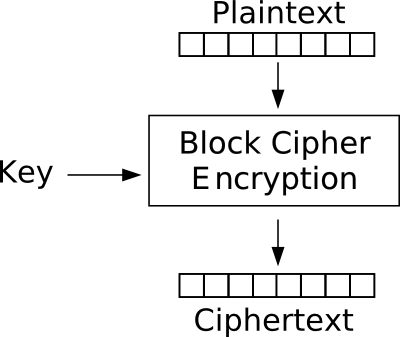
\includegraphics[width=4.5cm,height=3.5cm]{Encryption}
	 \end{minipage}
	 \hspace{.1\linewidth}
	 \begin{minipage}[b]{.4\linewidth}
		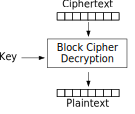
\includegraphics[width=4.5cm,height=3.5cm]{Decryption}
	 \end{minipage}
	\end{figure}
\end{frame}

\begin{frame}
\frametitle{structures of block ciphers}
	\begin{itemize}
		\item rounds
		\item feistel-network
		\item substitution-perumation-network
	\end{itemize}
\end{frame}

% ----

\begin{frame}
\frametitle{feistel-network}
	$L_{i+1} = R_i $ \\
	$R_{i+1} = L_i \oplus f(R_i, K_i)$
	\begin{center}
		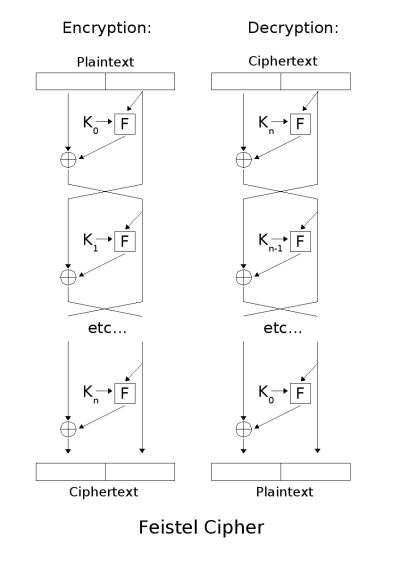
\includegraphics[scale=0.3]{Feistel}
	\end{center}
\end{frame}

%-----

\begin{frame}
\frametitle{S-Boxes}
	simple substituation function\\
	brings nonliearity\\
	mostly implemented as lookuptables
\end{frame}

%------

\begin{frame}
\frametitle{sample S-Boxe}
% \begin{tabular}{r|*{16}{r}}
%    &  0 &  1 &  2 &  3 &  4 &  5 &  6 &  7 &  8 &  9 & 10 & 11 & 12 & 13 & 14 & 15 \\ \hline
%  0 & 14 &  4 & 13 &  1 &  2 & 15 & 11 &  8 &  3 & 10 &  6 & 12 &  5 &  9 &  0 &  7 \\
%  1 &  0 & 15 &  7 &  4 & 14 &  2 & 13 &  1 & 10 &  6 & 12 & 11 &  9 &  5 &  3 &  8 \\
%  2 &  4 &  1 & 14 &  8 & 13 &  6 &  2 & 11 & 15 & 12 &  9 &  7 &  3 & 10 &  5 &  0 \\
%  3 & 15 & 12 &  8 &  2 &  4 &  9 &  1 &  7 &  5 & 11 &  3 & 14 & 10 &  0 &  6 & 13 \\
% \end{tabular}
 $S_1$ from DES:
 \begin{tabular}{c|*{16}{c}}
    &  0 &  1 &  2 &  3 &  4 &  5 &  6 &  7 &  8 &  9 &  A &  B &  C &  D &  E &  F \\ \hline
  0 &  E &  4 &  D &  1 &  2 &  E &  B &  8 &  3 &  A &  6 &  C &  5 &  9 &  0 &  7 \\
  1 &  0 &  F &  7 &  4 &  E &  2 &  D &  1 &  A &  6 &  C &  B &  9 &  5 &  3 &  8 \\
  2 &  4 &  1 &  E &  8 &  D &  6 &  2 &  B &  F &  C &  9 &  7 &  3 &  A &  5 &  0 \\
  3 &  F &  C &  8 &  2 &  4 &  9 &  1 &  7 &  5 &  B &  3 &  E &  A &  0 &  6 &  D \\
 \end{tabular}
\end{frame}

%-----







